\section{Nachrichtenaufbau}
\label{sec:Nachrichtenaufbau}
Jede Nachricht, die von dem Master-Computer (Raspberry Pi) gesendet und von dem 
OpenCM-Board korrekt empfangen werden soll, muss folgendes Format aufweisen:

Nachricht = \{ID\};\{COMMAND\};\{VALUE\};

Die Werte für \{ID\} sind für den entsprechenden Servomotor bestimmt und ist 
auf den Wertebereich zwischen 0 - 253 beschränkt.\\
Die Werte für \{COMMAND\} sind der Tabelle zu entnehmen, die auf folgender 
Website \url{} zu finden ist. Die wichtigsten Befehle sind zur Übrsicht in 
\ref{fig:commands} dargestellt.

\begin{figure}[H]
	\centering
	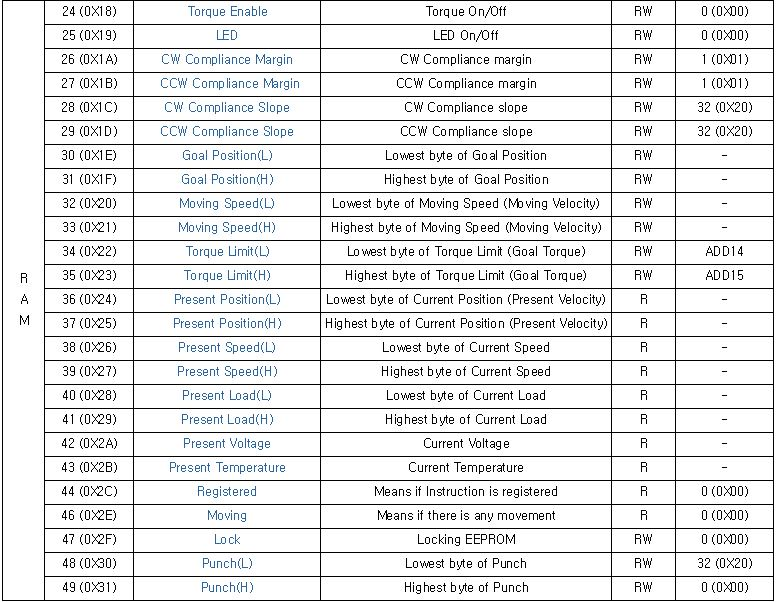
\includegraphics[width=0.85\textwidth]{03_Grafiken/Grundlagen/Nachrichtenaufbau/CommandsTable.jpg}
	\caption[Wichtige Kommandos]{Wichtige Kommandos}
	\label{fig:commands}
\end{figure}

Der Wert \{VALUE\} ist zunächst dafür vorgesehen, um den Drehwinkel für den 
Aktor angeben zu können. Um einen Servomotor mit der ID = 1 auf 55 $[$deg$]$ zu 
positionieren muss folgender String übertragen werden: \textbf{1;30;55;}

Auf dem übergeorndeten Rechner kann dann eine Regelstruktur implementiert 
werden, die entsprechende Kommandos an die jeweils beteiligten Aktoren sendet.
